%----------------------------------------------------------------------------------------
%	PACKAGES AND OTHER DOCUMENT CONFIGURATIONS
%----------------------------------------------------------------------------------------

\documentclass{article}

\usepackage{fancyhdr} % Required for custom headers
\usepackage{lastpage} % Required to determine the last page for the footer
\usepackage{extramarks} % Required for headers and footers
\usepackage[usenames,dvipsnames]{color} % Required for custom colors
\usepackage{pgf} % Required to insert pgf plots from matplotlib
\usepackage{graphicx} % Required to insert images
\usepackage{listings} % Required for insertion of code
\usepackage{courier} % Required for the courier font
\usepackage{lipsum} % Used for inserting dummy 'Lorem ipsum' text into the template
\usepackage[utf8]{inputenc}
\usepackage[ngerman]{babel}
\usepackage{multirow}

% Margins
\topmargin=-0.45in
\evensidemargin=0in
\oddsidemargin=0in
\textwidth=6.5in
\textheight=9.0in
\headsep=0.25in

\linespread{1.1} % Line spacing

% Set up the header and footer
\pagestyle{fancy}
%\lhead{\hmwkAuthorName} % Top left header
\chead{\hmwkClass\ : \hmwkTitle} % Top center head
\rhead{\firstxmark} % Top right header
\lfoot{\lastxmark} % Bottom left footer
\cfoot{} % Bottom center footer
\rfoot{Page\ \thepage\ of\ \protect\pageref{LastPage}} % Bottom right footer
\renewcommand\headrulewidth{0.4pt} % Size of the header rule
\renewcommand\footrulewidth{0.4pt} % Size of the footer rule

\setlength\parindent{0pt} % Removes all indentation from paragraphs

%----------------------------------------------------------------------------------------
%	CODE INCLUSION CONFIGURATION
%----------------------------------------------------------------------------------------

\definecolor{MyDarkGreen}{rgb}{0.0,0.4,0.0} % This is the color used for comments
\lstloadlanguages{Perl} % Load Perl syntax for listings, for a list of other languages supported see: ftp://ftp.tex.ac.uk/tex-archive/macros/latex/contrib/listings/listings.pdf
\lstset{language=Perl, % Use Perl in this example
        frame=single, % Single frame around code
        basicstyle=\small\ttfamily, % Use small true type font
        keywordstyle=[1]\color{Blue}\bf, % Perl functions bold and blue
        keywordstyle=[2]\color{Purple}, % Perl function arguments purple
        keywordstyle=[3]\color{Blue}\underbar, % Custom functions underlined and blue
        identifierstyle=, % Nothing special about identifiers                                         
        commentstyle=\usefont{T1}{pcr}{m}{sl}\color{MyDarkGreen}\small, % Comments small dark green courier font
        stringstyle=\color{Purple}, % Strings are purple
        showstringspaces=false, % Don't put marks in string spaces
        tabsize=5, % 5 spaces per tab
        %
        % Put standard Perl functions not included in the default language here
        morekeywords={rand},
        %
        % Put Perl function parameters here
        morekeywords=[2]{on, off, interp},
        %
        % Put user defined functions here
        morekeywords=[3]{test},
       	%
        morecomment=[l][\color{Blue}]{...}, % Line continuation (...) like blue comment
        numbers=left, % Line numbers on left
        firstnumber=1, % Line numbers start with line 1
        numberstyle=\tiny\color{Blue}, % Line numbers are blue and small
        stepnumber=5 % Line numbers go in steps of 5
}

% Creates a new command to include a perl script, the first parameter is the filename of the script (without .pl), the second parameter is the caption
\newcommand{\perlscript}[2]{
\begin{itemize}
\item[]\lstinputlisting[caption=#2,label=#1]{#1.pl}
\end{itemize}
}

%----------------------------------------------------------------------------------------
%	DOCUMENT STRUCTURE COMMANDS
%	Skip this unless you know what you're doing
%----------------------------------------------------------------------------------------

% Header and footer for when a page split occurs within a problem environment
\newcommand{\enterProblemHeader}[1]{
%\nobreak\extramarks{#1}{#1 continued on next page\ldots}\nobreak
%\nobreak\extramarks{#1 (continued)}{#1 continued on next page\ldots}\nobreak
}

% Header and footer for when a page split occurs between problem environments
\newcommand{\exitProblemHeader}[1]{
%\nobreak\extramarks{#1 (continued)}{#1 continued on next page\ldots}\nobreak
%\nobreak\extramarks{#1}{}\nobreak
}

\setcounter{secnumdepth}{0} % Removes default section numbers
\newcounter{homeworkProblemCounter} % Creates a counter to keep track of the number of problems

\newcommand{\homeworkProblemName}{}
\newenvironment{homeworkProblem}[1][Problem \arabic{homeworkProblemCounter}]{ % Makes a new environment called homeworkProblem which takes 1 argument (custom name) but the default is "Problem #"
\stepcounter{homeworkProblemCounter} % Increase counter for number of problems
\renewcommand{\homeworkProblemName}{#1} % Assign \homeworkProblemName the name of the problem
\section{\homeworkProblemName} % Make a section in the document with the custom problem count
%\enterProblemHeader{\homeworkProblemName} % Header and footer within the environment
}{
%\exitProblemHeader{\homeworkProblemName} % Header and footer after the environment
}

\newcommand{\problemAnswer}[1]{ % Defines the problem answer command with the content as the only argument
\noindent\framebox[\columnwidth][c]{\begin{minipage}{0.98\columnwidth}#1\end{minipage}} % Makes the box around the problem answer and puts the content inside
}

\newcommand{\homeworkSectionName}{}
\newenvironment{homeworkSection}[1]{ % New environment for sections within homework problems, takes 1 argument - the name of the section
\renewcommand{\homeworkSectionName}{#1} % Assign \homeworkSectionName to the name of the section from the environment argument
\subsection{\homeworkSectionName} % Make a subsection with the custom name of the subsection
%\enterProblemHeader{\homeworkProblemName\ [\homeworkSectionName]} % Header and footer within the environment
}{
%\enterProblemHeader{\homeworkProblemName} % Header and footer after the environment
}

%----------------------------------------------------------------------------------------
%	NAME AND CLASS SECTION
%----------------------------------------------------------------------------------------

\newcommand{\hmwkTitle}{Übung\ \#6} % Assignment title
\newcommand{\hmwkDueDate}{Montag,\ 01.\ Dezember\ 2014} % Due date
\newcommand{\hmwkClass}{Introduction to HPC} % Course/class
\newcommand{\hmwkClassTime}{} % Class/lecture time
\newcommand{\hmwkClassInstructor}{} % Teacher/lecturer
\newcommand{\hmwkAuthorName}{Günther Schindler, Christoph Klein, Klaus Naumann} % Your name

%----------------------------------------------------------------------------------------
%	TITLE PAGE
%----------------------------------------------------------------------------------------

\title{
\vspace{2in}
\textmd{\textbf{\hmwkClass:\ \hmwkTitle}}\\
\normalsize\vspace{0.1in}\small{Abgabe\ am\ \hmwkDueDate}\\
\vspace{0.1in}\large{\textit{\hmwkClassTime}}
\vspace{3in}
}

\author{\textbf{\hmwkAuthorName}}
\date{} % Insert date here if you want it to appear below your name

%----------------------------------------------------------------------------------------

\begin{document}

\maketitle

%----------------------------------------------------------------------------------------
%	TABLE OF CONTENTS
%----------------------------------------------------------------------------------------

%\setcounter{tocdepth}{1} % Uncomment this line if you don't want subsections listed in the ToC

\newpage
\tableofcontents
\newpage

%----------------------------------------------------------------------------------------
%	Heat Relaxation – Parallel Implementation
%----------------------------------------------------------------------------------------

\begin{homeworkProblem}[Parallel implementation based on 1D-row partitioning]

\end{homeworkProblem}
\pagebreak
%----------------------------------------------------------------------------------------
%	Heat Relaxation - Experiments
%----------------------------------------------------------------------------------------
\begin{homeworkProblem}[Heat Relaxation - Experiments]
In order to calculate the flops we determined the equation
\\
$FLOPS = (N^{2} - 4N + 4) \cdot 7$ , with N = grid-size.
\\
Following table shows the average time for different grid-sizes. The measured results
base on 50 to 10.000 iterations, depending on the used grid-size.\\
\begin{center}
\begin{tabular}{ |c|c|c|c|c|c|c| }
\hline 
Time / Iteration & NP & NP & NP & NP & NP & NP\\
\hline
Grid Size & 2 & 4 & 6 & 8 & 10 & 12\\
\hline
128x128 & 0.000196 & 0.000217 & 0.000079 & 0.000065 & 0.000094 & 0.000100\\ 
\hline
512x512 & 0.003130 & 0.001246 & 0.001260 & 0.003804 & 0.001596 & 0.001323\\ 
\hline
1024x1024 & 0.013285 & 0.004686 & 0.005300 & 0.005174 & 0.006413 & 0.006468 \\ 
\hline
2kx2k & 0.052558 & 0.018573 & 0.021031 & 0.016017 & 0.025776 & 0.026442 \\
\hline
4kx4k & 0.227757 & 0.093330 & 0.066810 & 0.056120 & 0.046239 & 0.044635 \\
\hline
\end{tabular}
\end{center}

\begin{center}
\begin{tabular}{ |c|c|c|c|c|c|c|c| }
\hline 
Time / Iteration & NP & NP & NP & NP & NP & NP & Sequential execution time\\
\hline
Grid Size & 2 & 4 & 6 & 8 & 10 & 12 &\\
\hline
128x128 & 0.311 & 0.281 & 0.772 & 0.938 & 0.649 & 0.610 & 0.000061\\ 
\hline
512x512 & 0.411 & 1.033 & 1.021 & 0.338 & 0.806 & 0.973 & 0.001287\\ 
\hline
1024x1024 & 0.549 & 1.555 & 1.375 & 1.408 & 1.136 & 1.127 & 0.007287\\ 
\hline
2kx2k & 0.563 & 1.592 & 1.406 & 1.846 & 1.147 & 1.118 & 0.029565\\
\hline
4kx4k & 0.501 & 1.224 & 1.71 & 2.035 & 2.470 & 2.559 & 0.114212\\
\hline
\end{tabular}
\end{center}

\begin{center}
\begin{tabular}{ |c|c|c|c|c|c|c| }
\hline 
Time / Iteration & NP & NP & NP & NP & NP & NP\\
\hline
Grid Size & 2 & 4 & 6 & 8 & 10 & 12 \\
\hline
128x128 & 0.156 & 0.070 & 0.129 & 0.117 & 0.0645 & 0.051 \\ 
\hline
512x512 & 0.206 & 0.258 & 0.170 & 0.042 & 0.081 & 0.081 \\ 
\hline
1024x1024 & 0.275 & 0.389 & 0.229 & 0.176 & 0.114 & 0.094 \\ 
\hline
2kx2k & 0.282 & 0.398 & 0.234 & 0.231 & 0.115 & 0.093 \\
\hline
4kx4k & 0.251 & 0.306 & 0.285 & 0.254 & 0.247 & 0.213 \\
\hline
\end{tabular}
\end{center}
The plot below shows the performance in GFLOP/s depending on the grid-size. As we can
see, the performance heavily depends on the grid-size between 128 and 1024. After a 
grid-size of 1024 the performance continues steady. The number of floating point 
operations doesn't realy affects the performance.
\begin{center}
%\includegraphics[width=0.6\columnwidth]{}
\end{center}
Due to that, we conclude that the program is memory bound and not computationally bound.
The bottleneck is once again the size of the cache. For every relaxation we theoretically
need at least twice the grid-size in the cache. If we haven't that much memory in
cache it leads to cache misses, which results in a main memory access with much longer
latency.
\end{homeworkProblem}
\pagebreak
%----------------------------------------------------------------------------------------
%	Heat Relaxation – Pre-considerations for parallelization
%----------------------------------------------------------------------------------------
\begin{homeworkProblem}[Heat Relaxation – Pre-considerations for parallelization]
The basic idea is to implement the program as an SPMD model.
In order to decompose this problem into sub-tasks, we partition the entire array and
distribute the slices to all tasks. Each task owns a portion of the total array.

2D is the more suitable way to partition because we need 2 dimensions for each grid 
calculation. 1D partition is also possible but needs much more communication. 

We choose to split the array in row-major order because in row-major order, the rows
of the array are contiguous in memory. It is important for performance when traversing
the array because accessing array elements that are contiguous in memory is faster than
accessing elements which are not, due to caching.
\begin{center}
%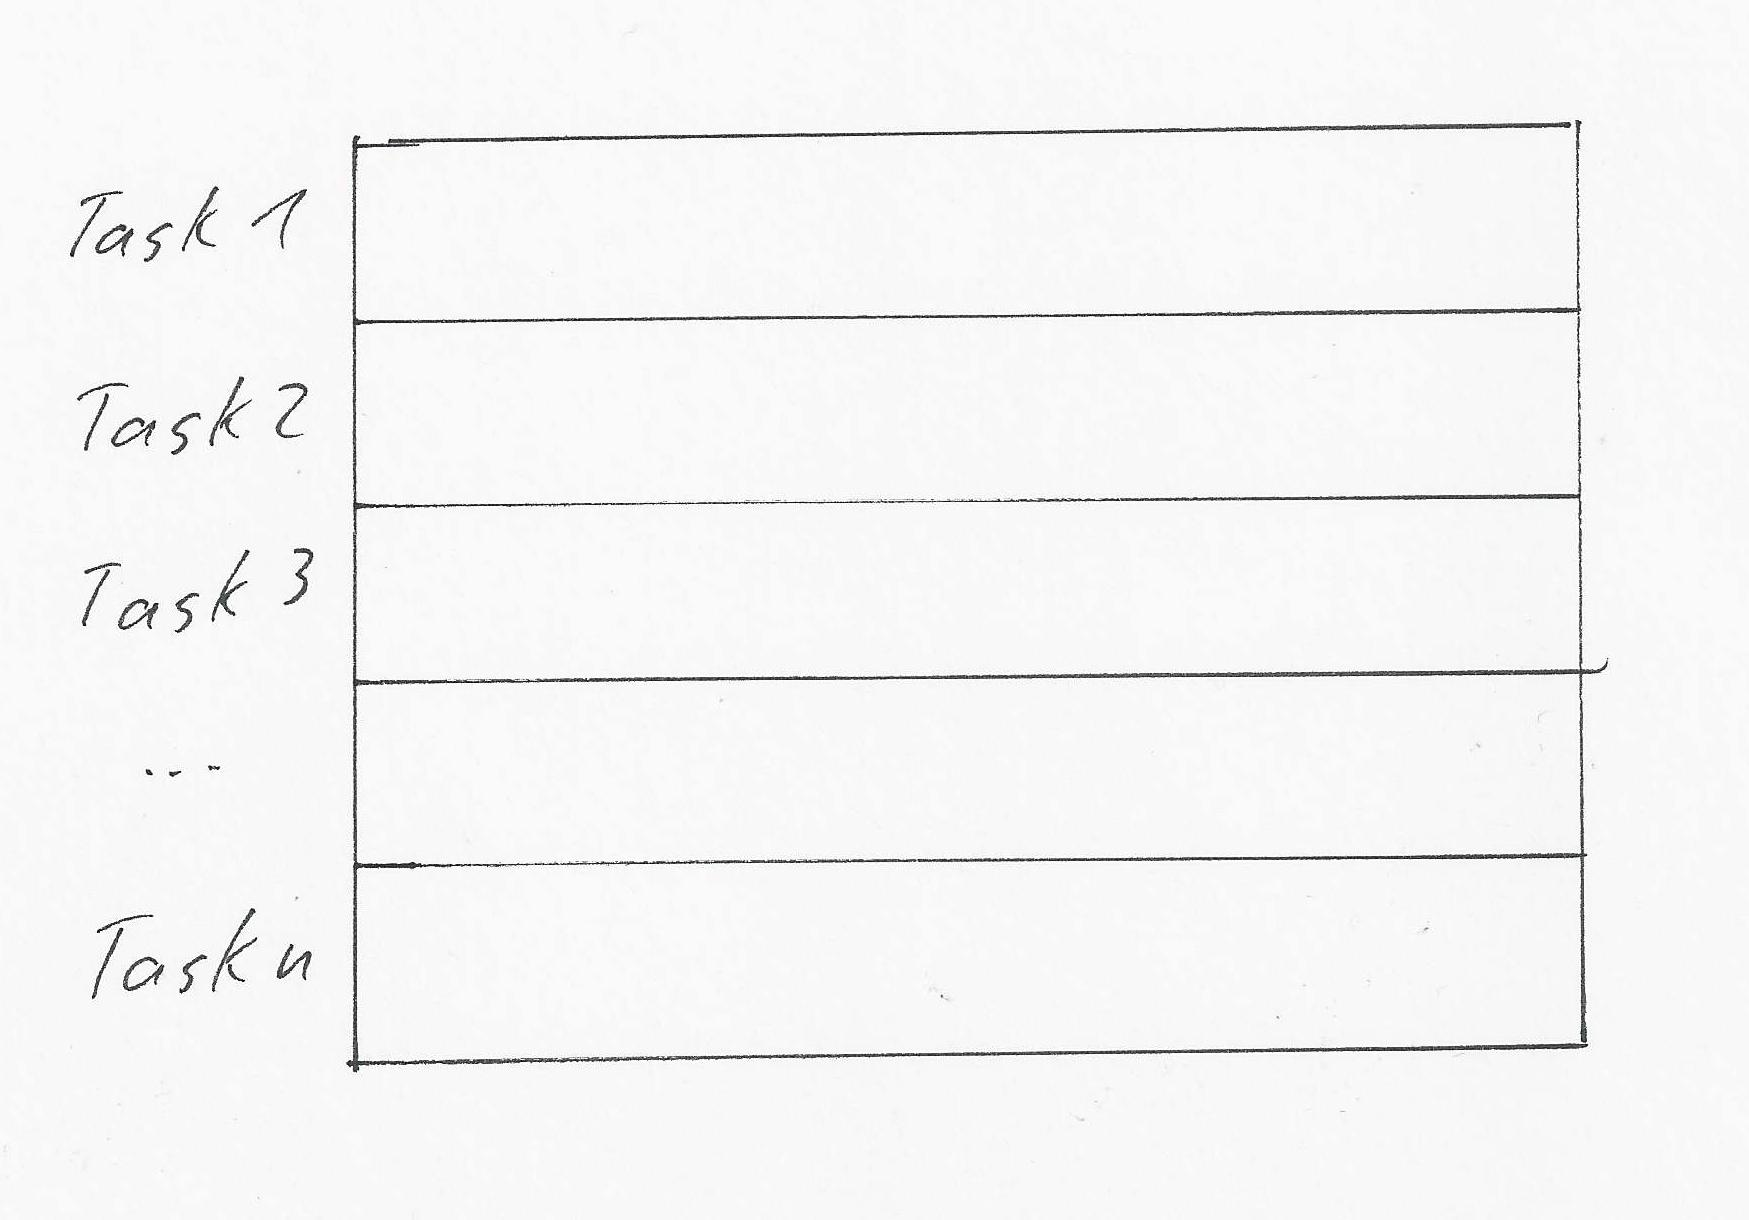
\includegraphics[width=0.6\columnwidth]{docu/image01-1.jpg}
\end{center}

The tasks depend on thier border rows. Interior-elements (1) belong to one task and 
are independent of other tasks. Border-elements (2) are dependent upon a neighbor 
task's data, so they need communication.
\begin{center}
%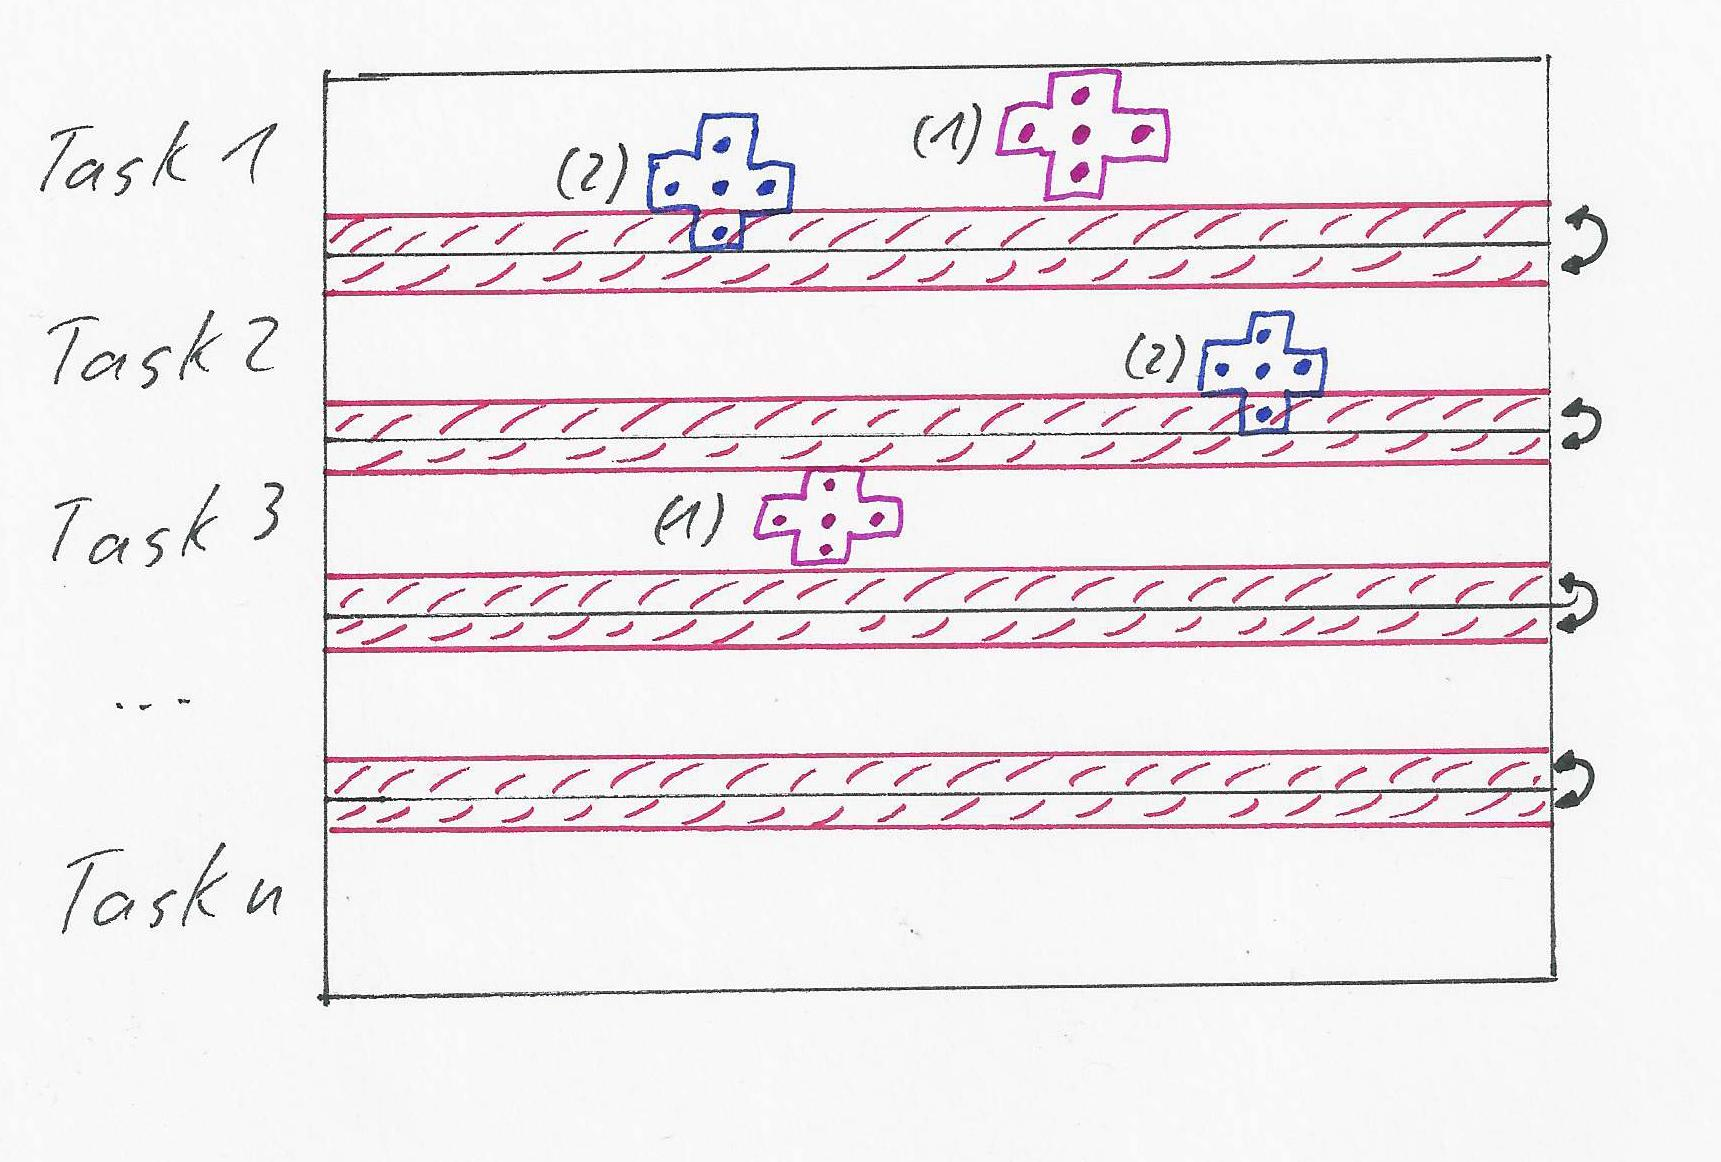
\includegraphics[width=0.6\columnwidth]{docu/image01-2.jpg}
\end{center}

We can use the independents of the interior-elements to hide latency and overlap 
computation and communication. Thus, we use non-blocking communication to exchange
data between the tasks. Each tasks sends its border-elements to it's neighbors, calculates
the interior-elements and gets, in the meantime, the border-elements of the neighbors.
After that, the task can calculate the border-elements as well.

To synchronize after each iteration, we use a barrier.
\end{homeworkProblem} 
\clearpage
\end{document}
